\documentclass[11pt]{report}

\usepackage[utf8]{inputenc}
\usepackage[francais]{babel}
\usepackage[T1]{fontenc}
\usepackage{graphicx}

\title{ Projet LO43 : SmallUTBM}
\author{Salomé \bsc{Welche} \& Romain \bsc{Dulieu} \& Haocheng \bsc{Xu} \& Romain \bsc{Thibaud}}
\date{Automne 2014}

\renewcommand{\contentsname}{Sommaire}

\begin{document}

\maketitle

\tableofcontents

\chapter{Introduction}

C'est dans le cadre de nos études à l'UTBM (Université de Technologie de Belfort-Montbéliard) que nous avons été amenés à déveloper une adaptation du jeu de plateau Smallworld\up{\copyright}. L'objectif du cours était d'introduire la programmation orientée objet grâce aux deux langages qui en sont les fers de lance, à savoir le C++ et le Java. C'est en Java que ce logiciel doit être programmé. 

Dans un premier temps, nous nous devons de bien assimiler les règles et les subtilités du jeu afin de pouvoir les traduire en langage informatique. De plus, une bonne compréhension de ces dernières est nécessaire pour pouvoir les adapter au mieux à l'univers qu'est l'UTBM. En effet, l'objectif est d'offrir une expérience pensée autour de ce qu'est la vie à l'UTBM.

Une fois cette première phase terminée, il est nécessaire d'effectuer une analyse technique et profonde du logiciel. Il est important d'effectuer cette expertise en amont pour faciliter l'implémentation future. Cette étape repose sur l'analyse UML mais aussi une réflexion autour de l'organisation du programme et des outils utilisés.

Enfin, nous entamons la phase de production. L'ensemble des tâches à effectuer est hiérarchisé afin de rendre une application la plus aboutie possible dans le temps imparti.

\chapter{Le jeu : Smallworld}

	\section{Description globale}
		Smallworld\up{\copyright} est jeu de plateau se jouant de 2 à 5 joueurs. C'est un jeu de stratégie militaire au tour par tour à la manière d'un Risk\up{\copyright}. L'originalité du jeu repose sur le fait que le plateau semble trop petit pour tout les joueurs et les unités trop peu nombreuses pour anéantir ses adversaires. Toute la subtilité repose alors sur la gestion d'un peuple de son avènement à l'extinction de ce dernier en passant bien entendu par son âge d'or. L'objectif est donc de gérer un peuple et de décider quand est-ce qu'il n'est plus rentable. On décide alors de le mettre en déclin et ensuite de choisir un nouveau peuple pour jouer avec. 
		
		Cette mécanique de jeu, qui demande au joueur d'être pragmatique, est amplifiée par une faible présence d'aléatoire dans les phases de combats. Au contraire de Risk\up{\copyright}, où il y a lancé de dé à chaque combat, le rapport de force s'effectue sur le nombre d'unité en présence, pour prendre un territoire adverse, il faut attaquer avec plus d'unité que la défense. Il y a cependant deux exceptions : lors de la dernière bataille d'un joueur il peut jeter un dé de renfort ou en cas de pouvoir spécial (qui sera détaillé plus tard).
		
		Bien que la stratégie de conquête soit au centre du gameplay, l'objectif n'est pas d'exterminer tous nos compagnons de jeu. La fin de la partie est déterminée par un nombre de tour par joueur. Le vainqueur étant celui qui a accumulé le plus de points de victoire. Ces mêmes points de victoire servant de monnaie durant la partie, il faut alors savoir évaluer la rentabilité de chaque coup. 
		
		De plus, la rejouabilité du jeu est assurée par l'unicité de chaque partie. En effet, tous les peuples n'étant pas accessibles à tout moment, le joueur doit s'adapter à chaque fois. A cela s'ajoute des pouvoirs qui sont aussi tirés aléatoirement et assignés à un peuple. Cette multiplicité de combinaisons peuple-pouvoir entraîne par contre une difficulté d'équilibrage qui se ressent de temps à autres, certaines alliances parraissant plus fortes que d'autres.
	\section{Règles du jeu}

\chapter{Adaptation des règles}

	\section{Ambiance recherchée}
	
	L'objectif étant seulement d'adapter l'univers heroic-fantasy du Smallworld\up{\copyright} à l'univers de l'UTBM, il n'y a pas de recherche sur le système de jeu à proprement dit. Sans ces notions de game design, nous nous sommes intéressés à la cosmétique du jeu pour installer notre ambiance. 
	
	Nous avons voulu jouer sur les petites rivalités qu'il peut exister, ou du moins qu'il semble exister entre les différentes instances de l'UTBM. Nous nous sommes appliqués à caricaturer ces rapports entre les différents corps de l'UTBM, en s'appuyant parfois sur des stéréotypes infondés mais quand même sympathiques. Notre volonté n'est pas de créer des clivages entre nos camarades. Nous avons d'ailleurs fait preuve d'autodérision par rapport aux instances auxquelles on appartient. 
	
	On a donc juste changé les noms des différents peuples, pouvoirs, ou encore élément de jeu. De temps à autres de petites modifications ont été apportées sur les mécaniques de jeu mais c'est essentiellement pour simplifier le passage sur informatique.    

	\section{Les peuples}
	
	Nous allons ici exposer les différents peuples en les liants à l'ancien peuple, la description du pouvoir et en expliquant pourquoi nous les avons choisi.
	
	\begin{description}
		\item[EDIM :] (ex Amazones). Les EDIMs commencent avec 4 pions supplémentaires, et tant qu'ils ont plus de 9 pions, ils perdent 2 pions par tour. Le clin d'oeil est ici fait à l'ancien peuple, car EDIM est le département avec le plus gros pourcentage de filles.
		\item[TC :] (ex Mi-portions). Les TCs ne peuvent rentrer que par le côté droit du plateau (coté Sévenans), ils installent alors leur premier appartement sur les deux premières régions conquises. Ces régions sont imprenables et immunisées. Quand on arrive en tronc commun, c'est souvent du lycée que l'on vient, et donc c'est la première expérience de vie indépendante pour la majorité, d'où le choix des plus petits êtres.
		\item[Administrarif :] (ex Nains) Tous les bureaux occupée par du personnel administratif (en déclin ou non) rapporte 1 UV supplémentaire en fin de tour. Les nains ayant un rapport particulier à l'argent, on les a mis en relations avec ceux qui gèrent le budget de l'UTBM.
		\item[Enseignants chercheurs :] (ex Elfes) Lorsqu'un adversaire s'empare d'une région, vous récupérez tous les pions de la région et les réorganisez sur les régions que vous occupez encore à la fin du tour. On a joué sur la rivalité elfes et orcs pour illustrer celle entre enseignants chercheurs et vacataires.
		\item[Vacataires :] (ex Orcs) Toute région conquise par des vacataires rapporte 1 UV supplémentaire à la fin du tour.
		\item[IMSI :] (ex Géant) Attaquez une région adjacente à un atelier coûte 1 unité de moins. Les IMSI étant les "pousse cartons", il fallait un peuple grand et fort pour les représenter.
		\item[Associatif :] (ex sorcier) A chaque tour, l'étudiant investit dans l'associatif peut remplacer un pion actif (seul) d'un autre peuple, adjacent à une région contrôlée par cet étudiant, par un pion associatif. L'associatif peut-être une raison d'échec à l'UTBM, c'est pourquoi il est en relation avec ceux qui pervertissent les autres peuples.
		\item[GMC :] (ex homme-rat) Pas de capacité spécifique, ils sont déjà l'élite (référence caricaturale aux discours de Mr Gomez).
		\item[Alternants :] (ex Humains) Toute case monde de l'entreprise occupée par vos alternants rapporte une UV supplémentaire en fin de tour. Cela montre la proximité entre alternants et entreprises.
		\item[EE : ] (ex Mages) Toute région comportant une source d'énergie rapporte une UV supplémentaire à la fin du tour. Le clin d'oeil semble évident (indice : ils étudient l'énergie).
		\item[Doctorants :] (ex Squelettes) Lors du redéploiement, rajoutez une unité par groupe de deux régions conquises ce tour-ci. Trois ans de plus à être étudiants, il y a de quoi devenir rachitique.
		\item[Etudiants Etranger :] (ex Tritons) Attaquez une région adjacente à une infrastructure de transport (gare, arrêt de bus,...) coûte 1 unité de moins. Ils remplacent les tritons car eux aussi viennent de contrées lointaines et inexplorées.
		\item[Info :] (ex Trolls) Placez une chambre avec un ordinateur sur chaque région occupée par des infos. La défense du territoire est augmenté de une unité, la chambre est détruite qu'à la disparition des infos de la région (elle reste en cas de déclin). Essayez de chasser un geek de devant son PC pour comprendre.
		\item[Décalé :] (ex Zombies) Lors du passage en déclin, toutes les unités restent sur le plateau et vous jouez normalement avec eux avant votre autre peuple. Les décalés sont ceux que les profs souhaitent virer mais qui s'accrochent.
	\end{description}

	\section{Les pouvoirs}
	Nous procédons de-même pour les pouvoirs :
	
	\begin{description}
		\item[Proche des entreprises : ] Tant que le peuple n'est pas en déclin, vous gagnez deux UVs supplémentaires à la fin de votre tour.
		\item[Fêtard : ]Toutes les régions nécessitent 1 unité de moins pour être envahies.
		\item[Drogué au café : ] A chaque fin de tour, choisissez deux régions et placez-y un thermos de café sur chaque, ces régions sont imprenables et immunisées.
		\item[Bilingues : ] Une fois par tour, placez un dictionnaire bilingue. Elle augmente la défense de la région de 1 et rapporte une UV supplémentaire à a fin de chaque tour (sauf si vous êtes en déclin). Elles disparaissent si vous quittez la région.
		\item[Grande Gueule : ] Vous pouvez jeter le dé de renfort avant de choisir une région à envahir (à chaque fois).
		\item[Qui sèche : ]Vous pouvez poursuivre votre expansion et passer en déclin juste après.
		\item[Connecté : ] Toutes les régions qui comptent une prise RJ45 sont considérées comme adjacentes pour vous. Ces régions nécessitent 1 unité de moins pour être envahie.
		\item[Et leur prof suiveur : ] Vous pouvez envahir une région avec une seule unité, une seule fois par tour. Placez alors le prof suiveur sur cette région, elle est imprenable et immunisée jusqu'à ce que le prof suiveur aille faire du soutient dans une autre région.
		\item[Des amphis : ] Prenez une UV supplémentaire pour chaque région avec un amphithéâtre à chaque fin de votre tour.
		\item[Des salles info : ] Prenez une UV supplémentaire pour chaque région avec une salle info à chaque fin de tour.
		\item[Des lieux de vie : ] Prenez une UV supplémentaire pour chaque région avec un lieu de vie à chaque fin de tour.
		\item[Fayots : ] Choisissez un adversaire que vous n'avez pas attaqué ce tour-ci, il ne pourra pas vous attaquer pendant son tour.
		\item[Avec équivalences : ] A la fin de votre premier tour, prenez 7 UV supplémentaires.
		\item[En double filière : ] Prenez une UV supplémentaire pour chaque région que vous occupez en fin de tour.
		\item[Du club Welcome : ] Vous pouvez envahir les infrastructures de transport.
		\item[Ponctuel : ] Les régions amphithéâtre et entreprises nécessitent 1 unité de moins pour être envahie.
		\item[Du père 200 : ] Toute région non vide conquise rapporte une UV supplémentaire à la fin du tour.
		\item[Revenant d'Erasmus : ] Vous pouvez conquérir n'importe quelle région, même une région non adjacente.
	\end{description}
	
\chapter{Analyse des problèmes}

	\section{Organisation globale du logiciel}

		\subsection{Gestion du projet}
			Tout d'abord, parmi les étudiants travaillant sur le projet, il y a un étudiant chinois. Pour faciliter la communication entre nous, nous avons donc décidé de travailler en anglais. C'est pourquoi, toute les productions liées à ce projet sont en anglais, mis à part les rapports (ça lui permet aussi de travailler son français). 
			
			Pour facilliter le travail en groupe nous avons aussi mis en place un gestionnaire de version, à savoir Git. Hébergé sur GitHub\up{\copyright}, cela permet de travailler en simultané sur le projet sans se marcher dessus, et d'avoir des sauvegardes des différentes phases de notre projet en cas de bug.
			
			D'un point vu logiciel, nous avons utilisé ArgoUML comme AGL (pour la création des diagrammes UML) et Eclipse comme IDE pour la programmation en java. Etant donné que nous avons effectué les diagrammes UML en amont, nous avons pu générer la structure du code via ArgoUML, et nous n'avons plus qu'à remplir les fonctions.
			
			Concernant la répartition des tâches, Romain T. s'occupe de la partie interface pendant que Salomé, Haocheng et Romain D. s'occupe de la conception du programme. Ils se sont occupés de construire les diagrammes UML auparavant. Ce rapport étant, lui, un produit collégial.
			
			
		\subsection{Structure du logiciel}
		
			Nous avons adopté pour ce projet un patron modèle-vue-contrôleur. La force de ce paradigme est d'être très modulable. En effet, il fonctionne en séparant l'interface du corps du programme et les fait dialoguer via un contrôleur. L'avantage est que si on change le type de la base de données par exemple, cela n'auras que très peu d'impact sur l'interface. 
			
			De plus, il est plus simple pour nous de travailler dessus, le code étant plus aéré et bien segmenté, nous pouvons plus facilement nous répartir le travail, et donc être plus efficaces. 

	\section{Le diagramme de cas d'utilisation}
	
	Nous avons commencé l'étude UML par un diagramme de cas d'utilisation.
Cela nous paraissait nécessaire pour comprendre quels intéractions avec l'utilisateur nous devrons implementer. 

Dans ce jeu il y 3 joueurs mais seulement 1 seul d'entre eux peut effectuer des actions durant son tour de jeu.
Il peut effectuer 4 actions différentes en fonction de l'état du jeu et des choix du joueur.
Nous expliquerons dans le diagramme d'Etat transition le déroulement d'un tour. 
Les 4 actions représentés ici serons détaillés dans les diagrammes de séquence.

\begin{figure}[!h]
\centering
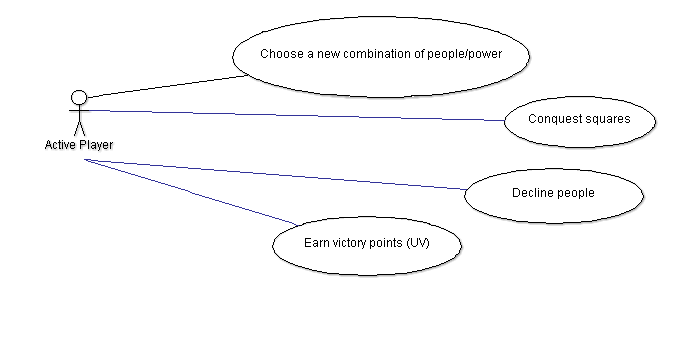
\includegraphics[width=13cm]{CasDutilisationPrincipal.png}
\caption{Diagramme de cas d'utlisation.}
\end{figure}

Nous n'avons pas beaucoup détaillé les actions dans ce diagramme mais malgré tout nous avons intégré certains détails qui nous paraissait importants.
Quand un joueur choisit une nouvelle combinaison de peuple/pouvoir cela peut conduire à une modifications au niveau des UV de ce joueur et des UV attribués aux peuple disponible.
Quand un joueur effectue une phase de conquête il va déplacer ses propres pions et détruire des pions adverses. Voir eventuellement rajouter d'autres types de pions sur le terrain.
Quand un joueur place son peuple actif en déclin cela va peut-etre lui faire perdre un ancien peuple et par conséquent de l'influence sur le terrain.
Au contraire l'action de compter et de recevoir des UV ne changera seulement le nombre d'UV possédé par le joueur actif.

	\section{Le diagramme d'état-transistion}
	
	Le diagramme d'Etat transition représente le déroulement d'un tour de jeu pour un joueur.
Chaque etat de ce diagramme correspond aux cas d'utilisation du programme et aux diagrammes de séquence.

\begin{figure}[!h]
\centering
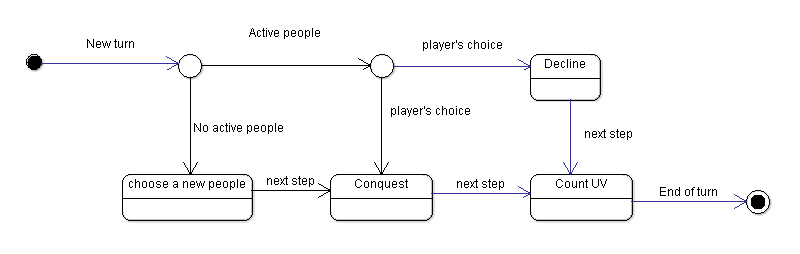
\includegraphics[width=13cm]{Tour.png}
\caption{Diagramme d'état transition.}
\end{figure}

Quand un joueur démarre un nouveau tour nous commençons tout d'abord par vérifier si il possède un peuple actif ou non.
Si il n'en possède pas (parce que c'est son premier tour de jeux ou qu'il vient de passer son peuple en déclin) Il doit alors choisir un nouveau peuple. Apres avoir récupérer une combinaison de peuple/pouvoir le joueur entame une phase de conquête pour installer son nouveau peuple sur le plateau de jeu.
Sinon le joueur devra faire un choix. Il doit maintenant choisir s'il veut continuer les conquêtes avec ce peuple ou s'il veut passer en déclin. 
Peu importe le choix que ce joueur aura fait, tous les tours doivent se terminer par un décompte des UV que le joueur gagne durant ce tour.

	\section{Les diagrammes de séquence}
	
	Nous avons choisi de faire des diagrammes de séquence pour montrer le déroulement d'un tour. Comme les tours diffèrent beaucoup suivant si on doit choisir un peuple ou si on passe en déclin, il paraît logique de faire deux diagrammes de séquences différents. Nous avons aussi fait les diagrammes de séquence de la conquête et de la récupération d'UVs car ces actions sont plutôt longues et se répètent à chaques tours.

		\subsection{Conquête}
		\begin{figure}[!h]
\centering
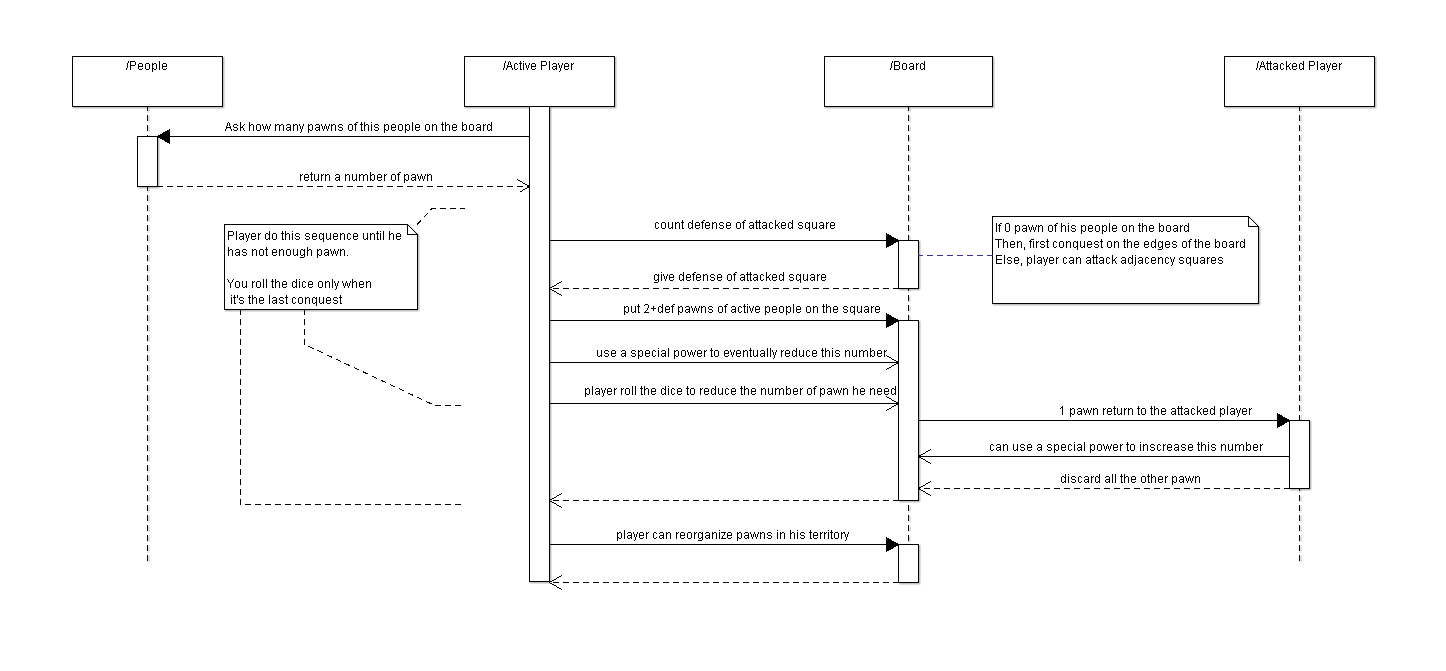
\includegraphics[width=13cm]{Conquetesequence.png}
\caption{Diagramme de séquence - phase de conquête.}
\end{figure}
		Pour le diagramme de séquence correspondant à la phase de conquête, nous avons deux acteurs (le joueur actif et le joueur attaqué) et deux éléments avec lesquels le joueur actif interagit. On doit d'abord vérifier si le joueur actif a déjà des pions de joué, si ce n'est pas le cas, sa première conquête doit se faire sur le bord du plateau. Le joueur doit ensuite compter la défense sur la case qu'il compte attaquer et s'il veut toujours l'attasuer, il pose un nombre de pions égal à la valeur de la défense à laquelle on ajoute deux. Ensuite, si le joueur a un pouvoir qui lui permettrait  de réduire le nombre de pions requis, il peut l'utiliser. Si c'est le dernier tour, le joueur peut aussi lancer un dé de renfort. Si la case attaquée appartenait à un autre joueur alors le joueur attaqué doit garder un des pions qui étaient sur la case et se défausser des autres s'il y en avait sauf s'il a un pouvoir qui lui permet d'augmenter le nombre de pions récupérés. Le joueur actif peut attaquer de nouvelles cases tant qu'il lui reste des pions en main. Quand il a fini d'attaquer, il peut réorganiser son territoire.

		\subsection{Déclin}
				\begin{figure}[!h]
\centering
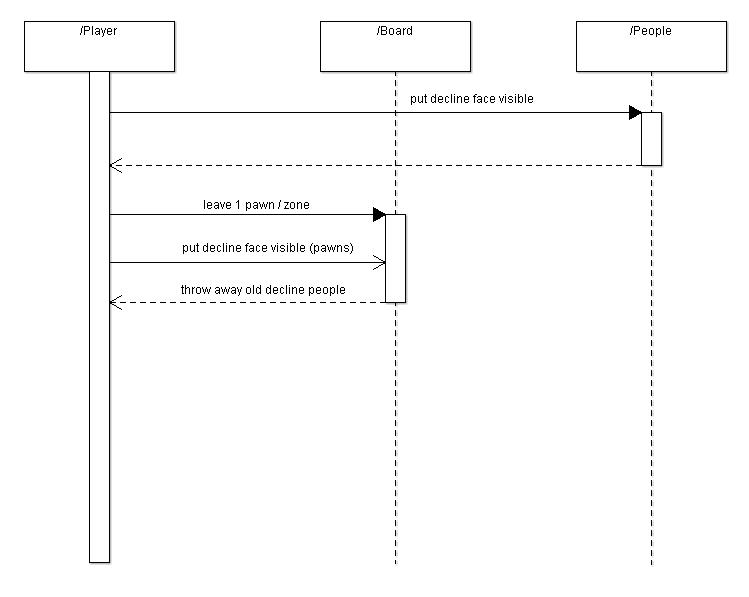
\includegraphics[width=13cm]{Declinsequence.png}
\caption{Diagramme de séquence - phase de déclin.}
\end{figure}
		Pour le diagramme correspondant au tour où le joueur choisit de passer en déclin, nous avons à nouveau un acteur qui est le joueur actif et deux éléments qui sont le plateau et le peuple associé à son pouvoir. Pendant le tour de déclin, le joueur met la face déclin de son peuple visible (ainsi que le pouvoir) et ne laisse qu'un pion par région occupée. Il doit ensuite retourner ses pions sur la face déclin et son tour est fini.

		\subsection{Nouveau peuple}
		
				\begin{figure}[!h]
\centering
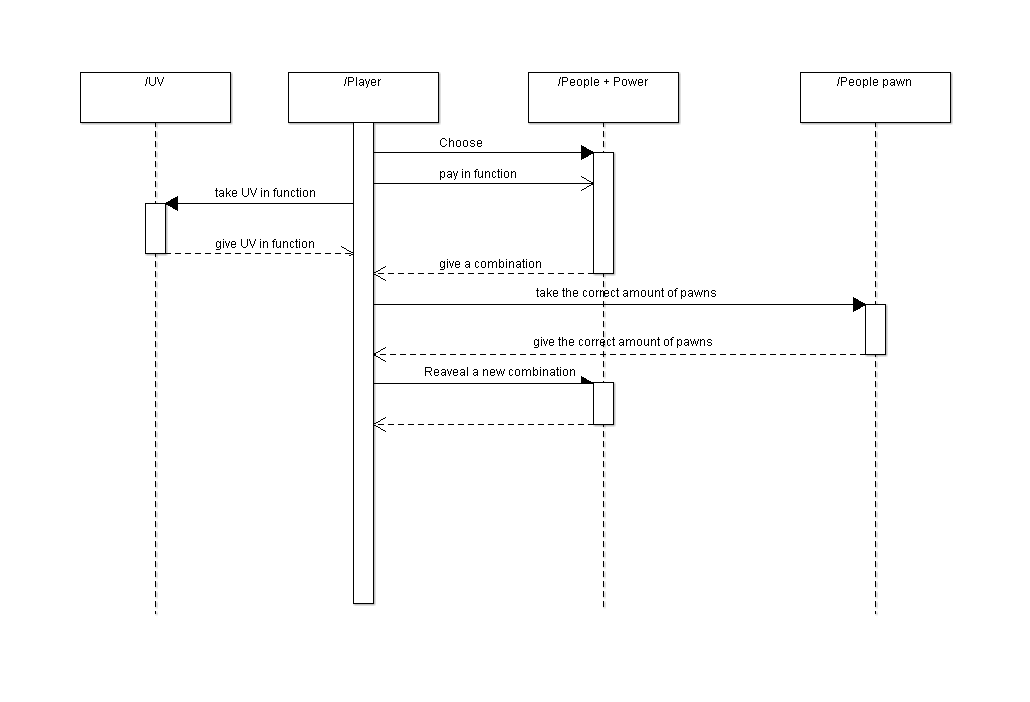
\includegraphics[width=13cm]{NouveauPeuplesequence.png}
\caption{Diagramme de séquence - phase de nouveau peuple.}
\end{figure}
		Pour le diagramme de séquence correspondant au tour où on choisi un nouveau peuple, en début de partie ou après avoir passé un peuple en déclin, nous avons mis un acteur (le joueur actif) et trois éléments avec lesquels il interagit. D'après les règles, le joueur choisit un peuple avec son pouvoir, paie le nombre d'UV approprié (si c'est le 2ème choix, on doit mettre une UV sur le peuple qui correspond au 1er choix) et récupère les UV sur son peuple s'il y en a. Une fois le peuple choisi, le joueur doit récupérer le bon nombre de pions suivant les nombres indiqués par le peuple et par le pouvoir. Enfin, le joueur remet la pioche correctement et le tour est terminé.

		\subsection{Gestion des UVs}
				\begin{figure}[!h]
\centering
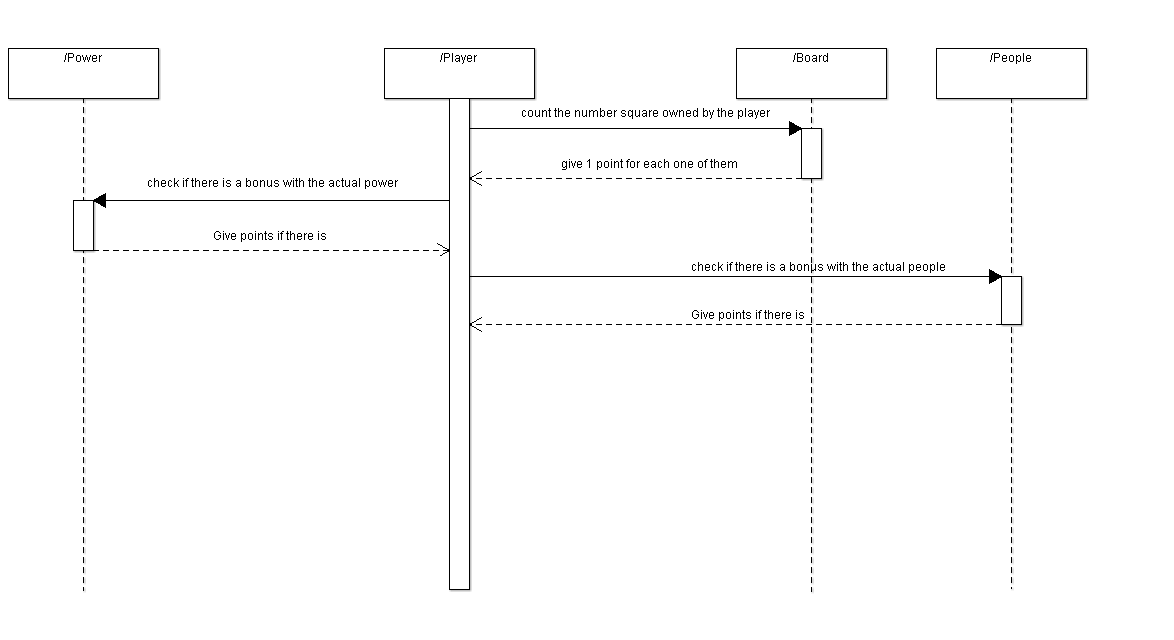
\includegraphics[width=13cm]{Pointssequence.png}
\caption{Diagramme de séquence - phase de récolte d'UVs.}
\end{figure}
		Pour le diagramme correspondant à la récupération d'UVs, nous avons un acteur qui est à nouveau le joueur actif et 3 éléments. Le joueur compte le nombre de zones qu'il occupe et récupère une UV par zone. Ensuite, il regarde si il a un pouvoir qui lui augmente son nombre d'UV récupéré. Enfin, il fait de même avec le peuple actif.

	

\chapter{Le modèle}

	\section{Le diagramme de classe du modèle}
	
	Notre diagramme de classe possède 13 classes et comme il y a beaucoup de méthodes on a choisi de mettre les plus importantes. Tous les constructeurs sont crées pour chaque classe par un AGL. Les cardinaux sont parfois des estimations car ils peuvent changer suivant les parties et le nombre de joueurs (par exemple on ne peut pas savoir en avance combien de pions on aura). 
	
	La première partie comporte les classes qui se rapporte au fonctionnement général du jeu tandis que la deuxième partie comporte les classes qui permettent de gérer le plateau de jeu.
Certaines classes sont représentés dans un rectangle aux bords épais car ils appartiennent a l'autre partie du diagramme mais isl possédent un lien avec la partie représenté.

					\begin{figure}[!h]
\centering
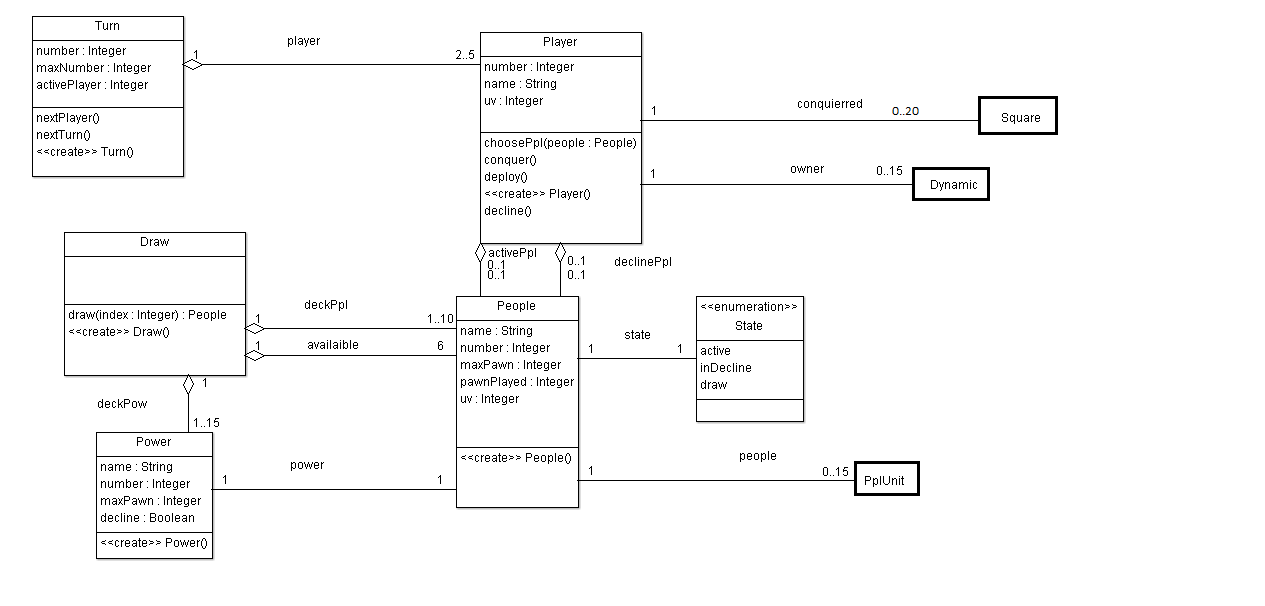
\includegraphics[width=13cm]{Game.png}
\caption{Diagramme de classe première partie.}
\end{figure}

\begin{description}


\item[Turn] : La classe Turn est la classe qui gère les tours. Il contient un numéro, un numéro maximal, un tableau de Player et le joueur actif représenté par un int. Cette classe va s'occuper des joueurs pour que tout les joueurs jouent une fois par tour puis il incrémente son numéro jusqu'à atteindre son numéro maximal où le dernier tour se joue.

\item[Player] : La classe Player correspond au joueur. Cette classe contient un nombre qui représente le joueur, un nom que le joueur choisit lui-même, un attribut uv qui correspond au nombre de points de victoire, un tableau conquierred qui est un tableau de Square, et deux attributs de type People qui représentent le peuple en déclin et le peuple actif. Cette classe va gérer le choix du peuple, la conquête, le déploiement et le passage en déclin.

\item[People] : La classe People correspond au peuple. Elle contient un nom, un numéro qui représente les différents objets, un nombre maximum de pions, le nombre de pions joués, le nombre d'UVs qu'il y a sur l'objet, un pouvoir de type Power et un état de type State. Cette classe est la classe mère de tous les types de peuple (GI, E, ...).

\item[State] : La classe State correspond à l'état d'un peuple (Actif, en déclin ou dans la pioche). Cette classe est une énumaration.

\item[Draw] : La classe Draw correspond à la pioche. Elle contient une liste chaînée de type People qui contient tous les peuples, une liste chaînée de type Power qui contient tous les pouvoirs et un tableau de type People qui contient les peuples que les joueurs peuvent choisir. Cette classe gère la pioche donc elle la remet correctement lorsqu'un peuple est choisi.

\item[Power] : La classe Power correspond au pouvoir. Elle contient un nom, un numéro par lequel ses objets seront représentés, un nombre maximal de pions, un booléen qui renvoie si le pouvoir est en déclin ou pas. Cette classe est la classe mère de tous les types de pouvoirs (Du club Welcome, qui sèche ...)



\end{description}
				\begin{figure}[!h]
\centering
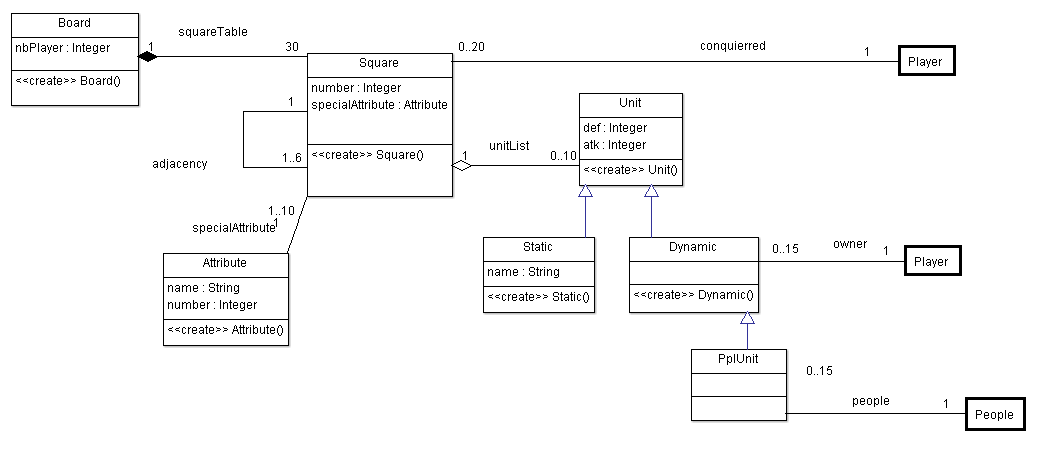
\includegraphics[width=13cm]{Board.png}
\caption{Diagramme de classe deuxième partie.}
\end{figure}
\begin{description}

\item[Unit] : La classe Unit correspond aux pions. Elle contient une valeur de défense et une valeur d'attaque.  Cette classe est la classe mère des classes Static et Dynamic.

\item[Board] : La classe Board correspond au plateau. Elle contient un entier qui représente le nombre de joueur. Nous utiliserons cet attribut car le plateau de jeu est différent suivant le nombre de joueurs.
Elle contient aussi un tableau de Square. C'est l'ensemble des cases qui compose le plateau de jeu. Dans le diagramme de classe nous avons écrit 30 cases mais ce nombre change en fonction du  nombre de joueur. 

\item[Square] : La classe Square correspond a une case du plateau de jeu. Elle contient un entier qui est l'indice de cet case. Une case peut avoir un attribut. C'est une particularité de la case qui sera utilisé par les pouvoirs des peuples.
Elle possède aussi un tableau de case pour référencer les autre cases qui lui sont adjacentes. Elle contient une liste d'unité qui représente les pions présents sur cette case. 

\item[Attribute] : La classe Attribute correspond aux différents attributs que les cases peuvent posséder. Elles ont un nom qui est une chaîne de caractère ainsi qu'un entier qui permet de les référencer plus facilement.

\item[Static] : La classe Statique est une enfant de Unit. Elle représente tous les pions qui ne peuvent pas bouger. Elle possède un seul attribut. Son nom, une chaîne de caractère.

\item[Dynamic] : La classe Dynamic est une enfant de Unit. Elle représente tous les pions qui peuvent bouger. Son seul attribut est une référence au joueur qui possède cette unité.

\item[PplUnit] : La classe PplUnit est une enfant de Dynamic. Elle représente les pions de peuple controllé par les joueurs. Elle possède en attribut une référence vers le peuple de cette unité.

\end{description}

	\section{Implémentation}
	Après avoir généré les classes à partir de l'AGL, nous avons enfin pu rentrer dans le vif du sujet. Pour commencer, nous avons choisi de considérer le fait que nous aurions 3 joueurs pour ne pas avoir à se soucier des différents plateaux.
	
	Ensuite, on a commencé à écrire les constructeurs et les méthodes principales. La classe Draw est presque complète et arrive a bien gérer la pioche. Nous avons aussi fait les écouteurs (listenners) sur le premières fenêtres (Demande du nombre de joueurs et l'entrée des noms des différents joueurs). 

\chapter{L'interface}

	\section{Description et organisation}
		Nous avons décidé de partitionné notre interface en 4 panneaux :
		\begin{description}
			\item[-]Un pour le plateaux de jeu
			\item[-]Un pour les actions du joueur
			\item[-]Un pour la pioche
			\item[-]Un pour rappeler l'ordre des actions
		\end{description}	
		
		Le plateau sera une image de fond avec des éléments clicables dessus où apparaitront les peuples. Les actions joueurs et la pioches ne seront que des éléments clicables, alors	que le panneau d'information ne sera qu'une succession d'élements textuels à caractères purement informatif.  
	\section{Solutions techniques}
		Nous avions commencer une implementation de l'interface en utlisant la bibliothèque graphique Swing. Mais cette bibliothèque ne nous convient pas assez, elle est lourde à mettre en place pour avoir des éléments dynamique, et elle n'est maintenu que pour des correctifs de bug, et donc ne propose plus d'avancées technologiques. 
		
		Pour ces raisons, nous sommes entrain d'étudier une migration vers JavaFX. De plus la communauté autour de cette bibliothèque semble très active sur le net, et donc offre un soutien et des tutoriels. Elle offre aussi la possibilité de travaillé avec des formats d'image en plus que ceux disponible sur swing (es : svg) permettant de travaillé avec des logiciels orienté vers l'image tel que Photoshop\up{\copyright}, Illustrator\up{\copyright}, ou encore Gimp\up{\copyright}. 
		
		Elle a aussi l'avantage d'être très portable (Linux, Mac, Windows, ou encore Android). Cela permet d'éventuellement penser à un portage multiplateforme.
\chapter{Prévisionnel des tâches}

	\section{Fonctionnement général}	
	
	Nous voulions avoir une démarche de projet correcte c'est donc pour cela que nous avons établi un prévisionnel des tâches pour suivre l'avancé du projet.
Le but de cette liste de tâches est d'obtenir un suivi correct et de vérifier que nous n'oublions aucune étape importante.
	\begin{description}
	\item Etude du problème
    \item Diagramme des cas d'utilisation
	\item Diagramme d'etat transition
	\item Diagrammes de séquence (4 diagrammes)
	\item Diagramme des classes
	\item Implémentation du modèle : 
	\item Système de pioche
	\item Impléntation du choix d'un nouveau peuple
	\item Impléntation de la classe Turn qui gère le fonctionnement d'un tour
	\item Impléntation d'un système de plateau (non rectangulaire)
	\item Implémentation du passage en déclin
	\item Impléntation des combats
	\item Impléntation du dé de renfort
	\item Impléntation du compte de point
	\item Impléntation d'un système qui détermine le vainqueur
	\item Lier le modèle et l'interface
	\item Gestion des pouvoirs
	\item Gestion des capacités des peuples
	\item Gestion des attributs des cases
	\end{description}

	\section{Interface}
	
	Il y a plusieurs tâches à effectuer :
	\begin{description}
	\item Une création et initialisation des panneaux
	\item Création des éléments clicables
	\item Rafraichissement de l'interface
	\item Gestion des cliquer-glisser
	\item Habillage de l'interface
	\item Création des cartes pour 2,4, et 5 joueurs
	\item Optimisation de la détection des régions
	\item Création d'animations
	
	\end{description}

\chapter{Conclusion}
	Ce projet est plutôt plaisant pour nous, vu notre inclinaison pour les jeux de plateux tel Smallworld\up{\copyright} (même si Seasons est mieux quand même). Il ne fut pas trop dur de nous impliquer dans l'analyse du jeu et son adaptation, ce fut même agréable et marrant.
	
	Au delà de l'aspect ludique du projet, nous avons pu découvrir ce qu'est un travail en équipe, car nous sommes quatre et que c'est la première fois que nous sommes autant dans un groupe. De plus, notre groupe est multiculturel. Nous avons donc du trouver des solutions afin d'être les plus efficaces possibles.
	
	Nous avons aussi mis en place des technologies que nous ne connaissions pas encore ou pas bien, ce qui est toujours enrichissant. Cependant, le temps d'adaptation nous à par contre parfois handicapé, et souvent ralentit.
	
	L'objectif était de finir ce rapport à 19h le vendredi 19 décembre et cela tombe bien, nous avons notre soirée jeu de plateaux en suivant. 
\end{document}